\documentclass[aspectratio=169,10pt]{beamer}

\usetheme{Madrid}
\usecolortheme{default}

\usepackage[UTF8,fontset=none]{ctex}
\setCJKmainfont{Noto Serif CJK SC}
\setCJKsansfont{Noto Sans CJK SC}
\setCJKmonofont{Noto Sans Mono CJK SC}
\usepackage{booktabs}
\usepackage{tabularx}
\newcolumntype{Y}{>{\raggedright\arraybackslash}X}
\newcolumntype{L}[1]{>{\raggedright\arraybackslash}p{#1}}
\usepackage{xcolor}
\usepackage{tikz}
\usepackage{graphicx}
\usetikzlibrary{positioning,arrows.meta,fit}

\definecolor{MainBlue}{RGB}{40,82,145}
\definecolor{AccentRed}{RGB}{178,56,46}
\definecolor{SoftGray}{RGB}{245,247,250}
\definecolor{DarkGray}{RGB}{70,76,86}
\definecolor{SoftGreen}{RGB}{232,246,238}
\definecolor{SoftYellow}{RGB}{255,247,222}

\setbeamercolor{title}{fg=white}
\setbeamercolor{frametitle}{fg=white,bg=MainBlue}
\setbeamercolor{block title}{bg=MainBlue,fg=white}
\setbeamercolor{block body}{bg=SoftGray,fg=black}
\setbeamercolor{alerted text}{fg=AccentRed}
\setbeamertemplate{navigation symbols}{}
\setbeamertemplate{footline}{}
\setbeamertemplate{headline}{}

\newcommand{\keypoint}[1]{\textbf{\textcolor{AccentRed}{#1}}}
\newcommand{\bluepoint}[1]{\textbf{\textcolor{MainBlue}{#1}}}

\title{SEW-Offload: 面向昇腾 NPU 的 MoE Expert Offloading}
\subtitle{Static Expert-Slot Windowing for Ascend MoE Offloading}
\author{}
\date{}

\begin{document}

\begin{frame}
  \titlepage
  \vspace{-1.0em}
  \begin{beamercolorbox}[wd=\linewidth,sep=0.75em,rounded=true]{block body}
  \centering
  \keypoint{不要把 NPU 当 GPU 用：}
  重点研究如何利用 Ascend 的差异化特性重塑 MoE expert offloading 的设计空间，并据此重新设计专家权重驻留、搬运、窗口化执行与预取机制。
  \end{beamercolorbox}
\end{frame}

\begin{frame}[t]{What is your problem}
\footnotesize
\vspace{-0.4em}

\bluepoint{问题背景}

\vspace{0.25em}
混合专家模型通过为每个 token 仅激活少量专家来扩展模型容量，但专家权重本身仍然给推理阶段的设备显存带来巨大压力。专家卸载因此成为在有限 HBM 条件下部署大规模 MoE 模型的重要路径。然而，现有 MoE offloading 系统大多沿用 GPU 时代的抽象，主要关注哪些专家应常驻显存、缺失专家何时从主机侧加载，以及如何进行专家缓存和预取。

\vspace{0.45em}
\begin{columns}[T]
\begin{column}{0.47\textwidth}
\textbf{\textcolor{MainBlue}{现有方法的 GPU 假设}}
\scriptsize
\begin{itemize}
  \item \textbf{expert caching：} 把 HBM 看作 expert cache，热 expert 常驻，冷 expert 放在 host；
  \item \textbf{host-to-device prefetching：} 根据历史路由或预测提前把可能需要的 expert 搬到设备；
  \item \textbf{CUDA stream overlap：} 依赖动态 kernel、stream 并发和异步拷贝隐藏传输开销。
\end{itemize}
\end{column}
\hfill
\begin{minipage}{0.45\textwidth}
\centering
\vspace{1.8em}
\textcolor{MainBlue}{\Large $\longrightarrow$} \\
\vspace{0.5em}
\textbf{\textcolor{AccentRed}{在 Ascend NPU 上}} \\
这些 GPU 时代的抽象 \\
\textbf{\textcolor{AccentRed}{不再完整}} \\
\vspace{0.5em}
$\downarrow$ 详见下页
\end{minipage}
\end{columns}

\vspace{0.7em}
\begin{beamercolorbox}[wd=\linewidth,sep=0.45em,rounded=true]{block body}
\textbf{\textcolor{AccentRed}{核心问题定义：}}
现有 MoE 卸载多把专家权重当作动态缓存对象，依靠替换、预取和拷贝/计算重叠来减少传输开销。但在 HBM 受限的昇腾 NPU 上，动态装载专家会破坏\textbf{稳定权重地址、固定执行窗口、图重放和显式搬运调度}。导致要么专家加载暴露在关键路径上，要么牺牲高效 NPU 执行所需的静态规整性。
\end{beamercolorbox}
\end{frame}

\begin{frame}[t]{Why it matters?}
\footnotesize
\vspace{-0.4em}

\bluepoint{MoE、Ascend 与 offloading 三个层面的必要性}

\vspace{0.3em}
随着 DeepSeek-V3/R1、Qwen-MoE、Mixtral 等模型普及，MoE 已成为大模型扩展的重要方向。问题不再只是能不能训练更大的模型，而是如何让超大 expert 参数在真实硬件上高效服务。

\vspace{0.35em}

\begin{columns}[T,onlytextwidth]
\begin{column}{0.32\textwidth}
\begin{minipage}[t][0.34\textheight][t]{\linewidth}
\begin{block}{1. 为什么 MoE 很重要}
\scriptsize
\begin{itemize}
  \item \textbf{扩展参数规模：} 拥有巨大专家参数池，但每个 token 只激活少量 expert；
  \item \textbf{提高推理性价比：} 相比同等总参数 dense 模型，用稀疏激活降低单 token 计算量；
  \item \textbf{代表前沿趋势：} DeepSeek、Qwen、Mixtral 表明，大规模 MoE 已成为高能力模型的重要形态。
\end{itemize}
\end{block}
\end{minipage}
\end{column}

\begin{column}{0.32\textwidth}
\begin{minipage}[t][0.34\textheight][t]{\linewidth}
\begin{block}{2. 为什么 Ascend 上重要}
\scriptsize
\begin{itemize}
  \item \textbf{国产算力主战场：} 生产环境依赖 Ascend 910B/910C，MoE 能否跑好直接影响算力可用性；
  \item \textbf{不能只复制 GPU：} Ascend 更强调稳定地址、固定 shape、图重放和显式搬运调度；
  \item \textbf{需要 NPU-native 路线：} 把 MoE 适配 Ascend，才能释放 AIC/AIV/MTE 等硬件能力。
\end{itemize}
\end{block}
\end{minipage}
\end{column}

\begin{column}{0.32\textwidth}
\begin{minipage}[t][0.34\textheight][t]{\linewidth}
\begin{block}{3. 为什么 offload 重要}
\scriptsize
\begin{itemize}
  \item \textbf{HBM 直接卡部署：} 大 MoE expert 权重放不下单卡 HBM，必须有可用卸载路径；
  \item \textbf{GPU-style offload 不够：} expert cache/prefetch 会破坏稳定地址、固定窗口和图重放；
  \item \textbf{必须保住 NPU 效率：} 既要省 HBM，又要让权重加载、MTE 和 grouped MLP 规整调度。
\end{itemize}
\end{block}
\end{minipage}
\end{column}
\end{columns}

\vspace{5.5em}
\begin{beamercolorbox}[wd=\linewidth,sep=0.55em,rounded=true]{block body}
\scriptsize
\textbf{\textcolor{AccentRed}{核心动机：}}
MoE 决定了前沿模型的扩展方向，Ascend 决定了这些模型在国产算力上的落地能力；
而 Ascend expert offloading 决定了在 HBM 受限时，能否把“参数很大但激活稀疏”的 MoE 真正高效部署起来。
SEW-Offload 的价值正是在 Ascend 约束下，把动态 expert 工作集转化为可复用、可预取、可流水化的固定 slot 执行窗口。
\end{beamercolorbox}
\end{frame}

\begin{frame}[t]{Why existing work fails?}
\scriptsize
\vspace{-0.55em}

\bluepoint{现有工作各自解决了局部问题，但没有同时覆盖“Ascend + HBM 受限 + expert offload”。}

\vspace{0.3em}
\setlength{\tabcolsep}{3pt}
\renewcommand{\arraystretch}{1.13}
\begin{tabularx}{\linewidth}{L{0.15\linewidth}L{0.22\linewidth}L{0.30\linewidth}Y}
\toprule
\textbf{工作类型} & \textbf{代表工作} & \textbf{做法} & \textbf{现有不足} \\
\midrule
GPU MoE 卸载 &
MoE-Infinity；Fiddler &
将专家作为 GPU 缓存或 CPU-GPU 协同对象，利用激活轨迹、专家热度或执行策略决定缓存替换、预取和 CPU/GPU 分工。 &
优化目标主要是减少 CPU--GPU 传输并提高 GPU 利用率；默认动态专家对象、动态执行入口和流级重叠可以接受，未处理 Ascend 对稳定权重地址、固定窗口、图重放和 MTE 编排的要求。 \\
\midrule
Ascend 全量 MoE &
vLLM Ascend \texttt{AscendFusedMoE}；\texttt{npu\_grouped\_matmul} &
将路由结果整理成每个专家的 token 计数和 \texttt{group\_list}，再调用 Ascend 分组矩阵乘执行 MoE MLP。 &
默认专家权重已经全量驻留 HBM；没有主机侧专家存储、固定驻留位置、缺失专家预取与替换，也没有针对卸载缺失的分阶段执行。 \\
\midrule
非 Ascend NPU MoE &
NPUMoE &
面向 Apple ANE，将稠密和静态计算卸载到 NPU；动态路由、top-k、分散/聚集等不规则部分回退到 CPU/GPU，并用静态分层、分组执行和图常驻降低开销。 &
目标硬件、内存体系和运行时不同；解决的是 ANE 静态图与动态算子回退问题，不解决 Ascend 上主机到 HBM 的专家权重装载、稳定槽位入口和 MTE/Cube 流水。 \\
\bottomrule
\end{tabularx}
\setlength{\tabcolsep}{6pt}
\renewcommand{\arraystretch}{1.0}

\vspace{0.3em}
\begin{beamercolorbox}[wd=\linewidth,sep=0.45em,rounded=true]{block body}
\textbf{\textcolor{AccentRed}{研究空白：}}
缺少面向 Ascend 的 \textbf{HBM 受限专家卸载}：不改变路由器、top-k 和 token 语义，同时处理权重驻留、搬运隐藏和稳定执行入口。
\end{beamercolorbox}
\end{frame}

\begin{frame}[t]{What is your key idea?}
\footnotesize
\vspace{-0.65em}

\bluepoint{把目标从"提高 cache hit rate"改写为"最小化暴露在关键路径上的 stall"：}

\vspace{-0.1em}
\begin{center}
\begin{beamercolorbox}[wd=0.58\linewidth,sep=0.3em,rounded=true,center]{block body}
\footnotesize
\textbf{\textcolor{AccentRed}{优化目标：}}
$\displaystyle T_{\text{stall}} = \max\bigl(0,\; T_{\text{load-miss}} - T_{\text{overlap}}\bigr)$
\quad
\textcolor{DarkGray}{不是 hit rate 高就行，而是 miss 加载能否被计算覆盖}
\end{beamercolorbox}
\end{center}

\vspace{0.0em}
\begin{center}
\resizebox{0.98\linewidth}{!}{%
\begin{tikzpicture}[
  font=\footnotesize,
  challenge/.style={draw=AccentRed, fill=SoftYellow, rounded corners=2pt, text width=3.35cm, minimum height=1.15cm, align=center, inner sep=3pt},
  idea/.style={draw=MainBlue, fill=SoftGreen, rounded corners=2pt, text width=3.45cm, minimum height=1.75cm, align=center, inner sep=3pt},
  arrow/.style={-{Latex[length=2.6mm]}, very thick, color=MainBlue},
  pipearrow/.style={-{Latex[length=2.0mm]}, thick, color=DarkGray}
]
% Challenge row
\node[challenge] (c1) at (0,0) {\textbf{Challenge 1}\\[2pt]动态权重地址\\破坏 NPUGraph 重放\\与 Static Kernel 复用};
\node[challenge] (c2) at (4.8,0) {\textbf{Challenge 2}\\[2pt]按热度预取 $\rightarrow$ hit rate 高\\但 miss 专家加载仍可能\\暴露在关键路径上};
\node[challenge] (c3) at (9.6,0) {\textbf{Challenge 3}\\[2pt]等待所有 miss expert\\到齐再执行 $\rightarrow$ Cube 空闲,\\MTE 搬运与计算串行};

% Idea row
\node[idea] (i1) at (0,-2.35) {\textbf{Fixed Expert Slots}\\[3pt]HBM 预分配固定数量 slot,\\地址/形状/布局\textbf{永久不变};\\运行时只改 expert\_id $\rightarrow$ slot\_id,\\NPU 执行图始终看到稳定入口};
\node[idea] (i2) at (4.8,-2.35) {\textbf{Deadline-Aware Prefetch}\\[3pt]每次加载 = 带 deadline 的作业;\\按 \textbf{最晚就绪时间、影响 token 数、\\搬运代价}三维排序,\\紧迫且影响大的 expert 优先搬};
\node[idea] (i3) at (9.6,-2.35) {\textbf{Hit-First Phased Execution}\\[3pt]不等全部 expert 到齐:\\\textbf{Phase 0} 先执行 slot 中已就绪 experts,\\同时后台搬运 miss experts;\\\textbf{Phase 1} 再执行刚加载完的 experts};

% Arrows: challenge -> idea (drawn after all nodes defined)
\draw[arrow] (c1) -- (i1);
\draw[arrow] (c2) -- (i2);
\draw[arrow] (c3) -- (i3);

% Pipeline arrows between ideas
\draw[pipearrow] ([xshift=0.12cm]i1.east) -- node[above, font=\tiny, text=DarkGray]{稳定入口} ([xshift=-0.12cm]i2.west);
\draw[pipearrow] ([xshift=0.12cm]i2.east) -- node[above, font=\tiny, text=DarkGray]{调度结果} ([xshift=-0.12cm]i3.west);
\end{tikzpicture}
}
\end{center}

\vspace{-0.05em}
\begin{beamercolorbox}[wd=\linewidth,sep=0.4em,rounded=true]{block body}
\scriptsize
\textbf{\textcolor{AccentRed}{三层机制协同：}}
\textbf{① Fixed Slots} 提供 NPU 友好的稳定执行基底 $\rightarrow$ \textbf{② Deadline-Aware Prefetch} 决定谁先搬进 slot（最小化 $T_{\text{load-miss}}$）$\rightarrow$ \textbf{③ Hit-First Phased Execution} 用已有 expert 的计算覆盖剩余加载（最大化 $T_{\text{overlap}}$），最终将暴露 stall 压到最低。
\end{beamercolorbox}
\end{frame}

\iffalse
\small
\vspace{-0.4em}

\begin{columns}[T,onlytextwidth]
\begin{column}{0.49\textwidth}
\begin{block}{旧假设：expert cache 是主要问题}
\footnotesize
GPU MoE offloading 常把系统抽象成：
\begin{itemize}
  \item router 产生动态 expert 集合；
  \item runtime 根据热度/预测决定加载哪些 expert；
  \item expert kernel 对当前 batch 动态执行；
  \item cache 命中率和传输带宽决定性能。
\end{itemize}
\end{block}
\end{column}

\begin{column}{0.49\textwidth}
\begin{block}{在 Ascend 上缺失的约束}
\footnotesize
如果只复制 GPU cache 策略，会忽略：
\begin{itemize}
  \item graph capture 依赖稳定 tensor 形状和地址；
  \item static kernel 编译启动成本高，但重复执行收益大；
  \item MTE 搬运和 Cube 计算需要被流水化；
  \item 小而动态的 expert 执行会放大队列和调度开销。
\end{itemize}
\end{block}
\end{column}
\end{columns}

\vspace{0.8em}
\begin{beamercolorbox}[wd=\linewidth,sep=0.75em,rounded=true]{block body}
\textbf{\textcolor{AccentRed}{重新定义 offloading：}}
在 Ascend 上，offloading 不只是“expert 在 host 和 device 之间移动”，
还包括\textbf{权重驻留位置、slot 地址稳定性、图复用粒度、预取流水}这些 GPU 工作通常弱化的控制面。
\end{beamercolorbox}
\end{frame}

\begin{frame}[t]{Important correction: vLLM Ascend 已经做了什么}
\small
\vspace{-0.45em}

\bluepoint{我们不能把已有 grouped MoE 后端当成新贡献。}

\vspace{0.55em}
\begin{tabularx}{\linewidth}{p{0.24\linewidth}X X}
\toprule
\textbf{路径} & \textbf{已有机制} & \textbf{含义} \\
\midrule
MC2 & \texttt{npu\_moe\_distribute\_dispatch} 返回 \texttt{expert\_token\_nums} & dispatch 后已有每个 expert 的累计 token 边界 \\
AllGather & \texttt{npu\_moe\_init\_routing} 返回 \texttt{expert\_tokens} & token-level routing 被整理为 per-expert count \\
All2AllV & \texttt{torch.histc(topk\_ids)} 统计 \texttt{tokens\_per\_expert} & expert 粒度统计用于通信和 GMM \\
MLP & \texttt{npu\_grouped\_matmul(... group\_list=...)} & 后端按 expert 分组执行矩阵乘 \\
\bottomrule
\end{tabularx}

\vspace{0.85em}
\begin{beamercolorbox}[wd=\linewidth,sep=0.7em,rounded=true]{block body}
\textbf{\textcolor{AccentRed}{修正后的边界：}}
vLLM Ascend 已经解决了“per-token assignment 到 per-expert count/grouped execution”的表示问题。
SEW-Offload 不能声称这是贡献；我们的目标是在此基础上解决\alert{HBM 不足时 expert 权重不再全量常驻}的问题。
\end{beamercolorbox}
\end{frame}

\begin{frame}[t]{What is still missing: grouped count 不是 offloading window}
\small
\vspace{-0.45em}

\begin{columns}[T,onlytextwidth]
\begin{column}{0.48\textwidth}
\begin{block}{已有 grouped MoE 后端}
\footnotesize
\begin{itemize}
  \item 输入仍是每轮动态 \texttt{topk\_ids}；
  \item \texttt{group\_list} 的形状固定，但 count 数值动态；
  \item GMM 根据每轮 \texttt{split\_value} 决定 expert 的 M 维；
  \item 权重张量来自 \texttt{layer.w13\_weight/w2\_weight}。
\end{itemize}
\end{block}
\end{column}

\begin{column}{0.50\textwidth}
\begin{block}{Offloading 需要的新抽象}
\footnotesize
\begin{itemize}
  \item HBM 中只有固定数量 \texttt{expert\_slots}；
  \item \texttt{expert\_id -> slot\_id} 动态映射；
  \item slot 内权重 tensor 地址长期稳定；
  \item miss expert 触发加载、替换或慢速 fallback；
  \item slot 作为 graph/static-kernel 的稳定输入。
\end{itemize}
\end{block}
\end{column}
\end{columns}

\vspace{0.85em}
\begin{beamercolorbox}[wd=\linewidth,sep=0.72em,rounded=true]{block body}
\textbf{\textcolor{AccentRed}{关键差异：}}
grouped count 解决的是\textbf{activation 如何按 expert 执行}；
SEW-Offload 解决的是\textbf{expert 权重如何在 HBM 受限时以固定 slot 方式驻留、加载和复用}。
\end{beamercolorbox}
\end{frame}

\begin{frame}[t]{Opportunity: Ascend 给 MoE offloading 的新控制面}
\small
\vspace{-0.4em}

\begin{columns}[T,onlytextwidth]
\begin{column}{0.49\textwidth}
\begin{block}{Graph / static kernel}
\footnotesize
ACLGraph/NPUGraph 和 static kernel 更偏好固定 shape、固定 tensor 地址与有限执行变体。
这意味着 expert offloading 应该尽量让 device 侧权重入口稳定。
\end{block}

\begin{block}{AIC/AIV/MTE 分工}
\footnotesize
MoE 执行天然包含 routing、permute、grouped GEMM、combine 与权重搬运。
Ascend 的矩阵单元、向量单元和搬运单元让这些阶段有机会流水化。
\end{block}
\end{column}

\begin{column}{0.49\textwidth}
\begin{block}{Weight prefetch}
\footnotesize
vLLM Ascend 已经有通过额外 pipeline 预取线性层权重、降低 MTE 压力的经验。
Expert slot 可以把“预取哪些权重”变成显式策略问题。
\end{block}

\begin{block}{Fixed GM window}
\footnotesize
如果 NPU 侧只有固定数量 slot，且每个 slot 的权重布局固定，
runtime 可以把动态 expert 工作集翻译为稳定的 slot 执行窗口。
\end{block}
\end{column}
\end{columns}
\end{frame}

\begin{frame}[t]{Key idea: Static Expert-Slot Windowing}
\small
\vspace{-0.2em}

\begin{center}
\resizebox{0.96\linewidth}{!}{%
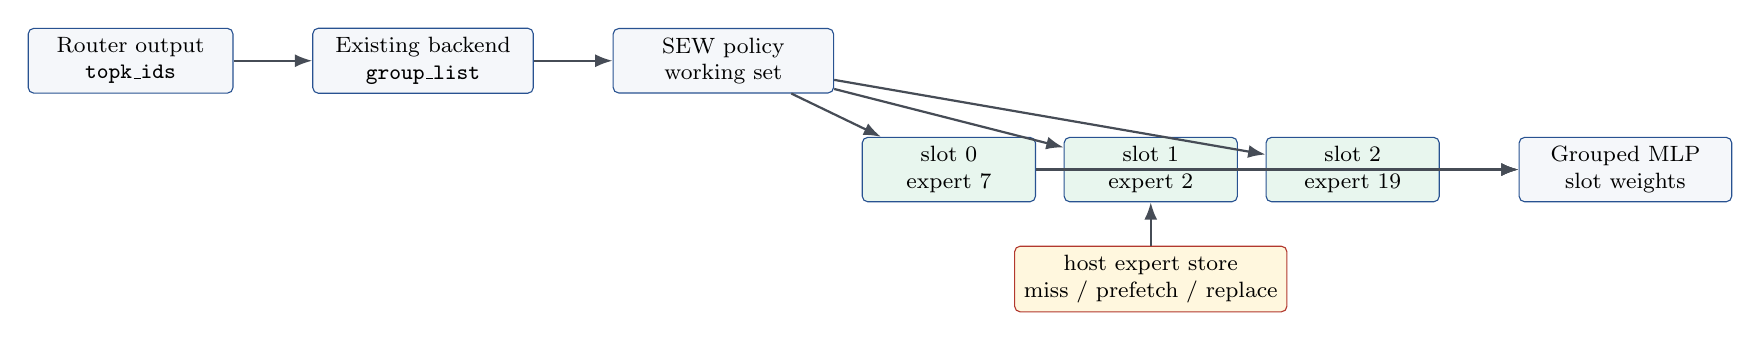
\begin{tikzpicture}[
  font=\footnotesize,
  node distance=0.9cm,
  box/.style={draw=MainBlue, fill=SoftGray, rounded corners=2pt, minimum height=0.75cm, align=center},
  slot/.style={draw=MainBlue, fill=SoftGreen, rounded corners=2pt, minimum height=0.72cm, align=center},
  miss/.style={draw=AccentRed, fill=SoftYellow, rounded corners=2pt, minimum height=0.72cm, align=center},
  arrow/.style={-{Latex[length=2.2mm]}, thick, color=DarkGray}
]
\node[box, minimum width=2.6cm] (router) {Router output\\\texttt{topk\_ids}};
\node[box, right=1.0cm of router, minimum width=2.8cm] (count) {Existing backend\\\texttt{group\_list}};
\node[box, right=1.0cm of count, minimum width=2.8cm] (policy) {SEW policy\\working set};
\node[slot, below right=0.55cm and 0.35cm of policy, minimum width=2.2cm] (slot0) {slot 0\\expert 7};
\node[slot, right=0.35cm of slot0, minimum width=2.2cm] (slot1) {slot 1\\expert 2};
\node[slot, right=0.35cm of slot1, minimum width=2.2cm] (slot2) {slot 2\\expert 19};
\node[miss, below=0.55cm of slot1, minimum width=3.4cm] (host) {host expert store\\miss / prefetch / replace};
\node[box, right=1.0cm of slot2, minimum width=2.7cm] (gmm) {Grouped MLP\\slot weights};

\draw[arrow] (router) -- (count);
\draw[arrow] (count) -- (policy);
\draw[arrow] (policy) -- (slot0);
\draw[arrow] (policy) -- (slot1);
\draw[arrow] (policy) -- (slot2);
\draw[arrow] (host) -- (slot1);
\draw[arrow] (slot2) -- (gmm);
\draw[arrow] (slot1) -- (gmm);
\draw[arrow] (slot0) -- (gmm);
\end{tikzpicture}
}
\end{center}

\vspace{0.55em}
\begin{beamercolorbox}[wd=\linewidth,sep=0.7em,rounded=true]{block body}
\textbf{\textcolor{AccentRed}{核心思想：}}
不改变 router 选出的 expert；只是在执行前，把 active expert 映射到固定数量、固定地址的 HBM slots。
命中的 expert 直接执行，未命中的 expert 触发加载/替换/降级路径。
\end{beamercolorbox}
\end{frame}

\begin{frame}[t]{Runtime abstraction}
\small
\vspace{-0.4em}

\begin{tabularx}{\linewidth}{p{0.24\linewidth}X X}
\toprule
\textbf{抽象} & \textbf{职责} & \textbf{为什么是 Ascend-specific} \\
\midrule
\texttt{ExpertStore} &
CPU/host 侧保存完整 expert 权重，支持按 expert 或 tile 加载 &
把 offloading 从一次性全量权重迁移变成可调度的数据搬运 \\
\texttt{SlotManager} &
维护固定数量 HBM slots 与 \texttt{expert\_id -> slot\_id} &
固定 slot tensor 地址，给 graph/static kernel 稳定入口 \\
\texttt{WindowPlanner} &
根据 \texttt{group\_list}、历史热度和 HBM budget 选择 resident set &
利用已有 per-expert count，而不是重新做 routing \\
\texttt{PrefetchEngine} &
在 routing/dispatch/GMM 间隙预取下一层或下一步 expert &
显式利用 MTE/权重预取流水，降低 Cube 等待 \\
\texttt{FallbackPath} &
处理 slot miss、超预算、预取失败和未覆盖 expert &
保证不 drop token，不改变模型语义 \\
\bottomrule
\end{tabularx}
\end{frame}

\begin{frame}[t]{One iteration data flow}
\small
\vspace{-0.35em}

\begin{enumerate}
  \setlength\itemsep{0.65em}
  \item \textbf{Routing：} 原始 router 产生 \texttt{topk\_ids/topk\_weights}，不修改激活结果。
  \item \textbf{Count extraction：} 复用现有 \texttt{token\_dispatcher.py} 得到 \texttt{group\_list/expert\_tokens}。
  \item \textbf{Working-set planning：} 根据当前层 active experts、历史局部性和 slot budget 决定 resident set。
  \item \textbf{Slot remap：} 将 active expert 映射到 \texttt{slot\_id}，构造 slot-local expert map。
  \item \textbf{Load/prefetch：} 对 miss expert 从 host store 加载到空闲或被替换 slot。
  \item \textbf{Grouped MLP：} 使用 slot 权重和现有 grouped matmul 路径执行。
  \item \textbf{Combine：} 复用现有 combine/unpermute，还原原始 token 顺序。
\end{enumerate}

\vspace{0.55em}
\begin{beamercolorbox}[wd=\linewidth,sep=0.7em,rounded=true]{block body}
\textbf{\textcolor{AccentRed}{语义保证：}}
SEW-Offload 只改变 expert 权重的驻留和访问方式，不改变 router logits、top-k expert、gate weight 或 combine 语义。
\end{beamercolorbox}
\end{frame}

\begin{frame}[t]{Integration in vLLM Ascend}
\small
\vspace{-0.35em}

\begin{columns}[T,onlytextwidth]
\begin{column}{0.54\textwidth}
\begin{block}{现有主路径}
\footnotesize
\begin{enumerate}
  \item \texttt{AscendFusedMoE.forward\_impl}
  \item \texttt{select\_experts}
  \item \texttt{build\_fused\_experts\_input}
  \item \texttt{moe\_comm\_method.fused\_experts}
  \item \texttt{token\_dispatch -> MLP -> combine}
\end{enumerate}
\end{block}
\end{column}

\begin{column}{0.44\textwidth}
\begin{block}{SEW 最小插入点}
\footnotesize
\begin{itemize}
  \item 在 \texttt{fused\_experts} 前准备 slot weights；
  \item 不改 scheduler；
  \item 不改 model runner；
  \item 不重写 token dispatcher；
  \item 默认关闭，通过配置开关启用。
\end{itemize}
\end{block}
\end{column}
\end{columns}

\vspace{0.7em}
\begin{beamercolorbox}[wd=\linewidth,sep=0.7em,rounded=true]{block body}
\textbf{\textcolor{AccentRed}{低侵入原则：}}
SEW-Offload 应作为 \texttt{vllm\_ascend/moe\_offload/} 中的独立 runtime，
通过薄 hook 接入 MoE boundary；现有 grouped count、dispatch、GMM 和 combine 尽量复用。
\end{beamercolorbox}
\end{frame}

\begin{frame}[t]{Policy design}
\small
\vspace{-0.4em}

\begin{columns}[T,onlytextwidth]
\begin{column}{0.33\textwidth}
\begin{block}{MVP-0: observe}
\footnotesize
\begin{itemize}
  \item 记录每层 active experts；
  \item 记录 \texttt{expert\_tokens}；
  \item 分析 temporal locality；
  \item 不改变执行路径。
\end{itemize}
\end{block}
\end{column}

\begin{column}{0.33\textwidth}
\begin{block}{MVP-1: sync slot}
\footnotesize
\begin{itemize}
  \item 固定 HBM slot 数；
  \item miss 同步加载；
  \item LRU/heat replacement；
  \item 保证 correctness。
\end{itemize}
\end{block}
\end{column}

\begin{column}{0.31\textwidth}
\begin{block}{MVP-2: prefetch}
\footnotesize
\begin{itemize}
  \item 基于上一层/上一 token 预测；
  \item 对下一层 hot expert 预取；
  \item overlap routing/dispatch；
  \item 统计 stall 与命中。
\end{itemize}
\end{block}
\end{column}
\end{columns}

\vspace{0.75em}
\begin{block}{MVP-3: graph-friendly window}
\footnotesize
将 slot 数、capacity tier 和权重入口固定成少量变体，
探索 ACLGraph/static kernel 对 offloaded expert path 的收益和限制。
\end{block}
\end{frame}

\begin{frame}[t]{Experiment plan}
\small
\vspace{-0.35em}

\begin{tabularx}{\linewidth}{p{0.20\linewidth}X}
\toprule
\textbf{维度} & \textbf{设计} \\
\midrule
模型 & Qwen3-30B-A3B；优先单机单卡，后续扩展多卡 expert parallel 对照 \\
场景 & 人工限制 resident expert slots，模拟 HBM 不足；保留真实 KV cache 压力 \\
Baseline 1 & vLLM Ascend 原生 grouped MoE，全量 expert 常驻 \\
Baseline 2 & 简单 LRU expert cache，无固定 slot/graph 设计 \\
Baseline 3 & GPU-style prediction/prefetch 思路移植，不做 Ascend-specific slot 稳定化 \\
SEW variants & sync slot、prefetch slot、capacity-tier slot、graph replay slot \\
Workloads & decode-heavy、mixed prefill/decode、长上下文、多请求连续批处理 \\
\bottomrule
\end{tabularx}
\end{frame}

\begin{frame}[t]{Metrics and ablations}
\small
\vspace{-0.35em}

\begin{columns}[T,onlytextwidth]
\begin{column}{0.49\textwidth}
\begin{block}{主要指标}
\footnotesize
\begin{itemize}
  \item end-to-end throughput；
  \item TTFT / TPOT / p95 latency；
  \item HBM peak / resident expert memory；
  \item slot hit rate / miss penalty；
  \item H2D bytes and stalls；
  \item graph replay hit rate；
  \item MTE/Cube overlap。
\end{itemize}
\end{block}
\end{column}

\begin{column}{0.49\textwidth}
\begin{block}{消融实验}
\footnotesize
\begin{itemize}
  \item slot 数量：2/4/8/16；
  \item replacement：LRU、LFU、token-count weighted；
  \item prefetch：无、上一层、上一 token、混合；
  \item capacity tier：关闭/少量 bucket；
  \item graph：eager、ACLGraph、static kernel。
\end{itemize}
\end{block}
\end{column}
\end{columns}
\end{frame}

\begin{frame}[t]{Expected claims}
\small
\vspace{-0.4em}

\begin{enumerate}
  \setlength\itemsep{0.85em}
  \item \textbf{表示层 claim：}
  Ascend grouped MoE 已经提供 per-expert count；offloading 应复用这个信号，而不是重新设计 routing。
  \item \textbf{系统层 claim：}
  固定 expert-slot residency 能让 HBM 受限 MoE offloading 保持稳定权重入口，减少动态权重对象破坏图复用的问题。
  \item \textbf{硬件层 claim：}
  slot 化后，expert load/prefetch 可以与 routing、dispatch、GMM 形成更明确的流水，有机会改善 MTE/Cube overlap。
  \item \textbf{语义层 claim：}
  SEW-Offload 不修改 router、不减少 expert 激活、不做 drop，因此 correctness 风险低于重路由或容量裁剪方法。
\end{enumerate}
\end{frame}

\begin{frame}[t]{Risks and fallback}
\small
\vspace{-0.4em}

\begin{tabularx}{\linewidth}{p{0.28\linewidth}X X}
\toprule
\textbf{风险} & \textbf{表现} & \textbf{应对} \\
\midrule
slot miss 太多 & 加载阻塞吞吐，尾延迟升高 & decode/prefill 分开评估；引入 token-count weighted replacement \\
graph 收益有限 & dynamic count 仍导致图变体过多 & 先固定权重 slot 地址，再逐步引入 capacity tier \\
H2D 搬运太慢 & offload 节省 HBM 但拖慢计算 & 量化 expert store、tile-level prefetch、异步加载 \\
工程侵入过大 & 影响 vLLM Ascend 主路径稳定性 & 默认关闭；新包封装；先 observer，再 sync slot \\
正确性难验证 & slot remap 引入 expert 对错风险 & 保留 expert-id checksum、逐层输出对齐、E2E replay 测试 \\
\bottomrule
\end{tabularx}
\end{frame}

\begin{frame}[t]{Roadmap}
\small
\vspace{-0.4em}

\begin{block}{Phase 1: Trace and evidence}
\footnotesize
实现 routed expert working-set 记录，得到 Qwen3-30B-A3B 在真实 workload 下的 expert locality、active set size、layer-to-layer overlap。
\end{block}

\begin{block}{Phase 2: Minimal offloading}
\footnotesize
构建 host expert store 与固定 HBM slots，先用同步加载跑通 correctness，
证明在人工 slot budget 下能替代全量 expert 常驻。
\end{block}

\begin{block}{Phase 3: Ascend-specific optimization}
\footnotesize
加入 slot prefetch、capacity tier 和 graph/static-kernel 实验，
验证固定 slot 地址是否能提升 replay 稳定性并降低搬运 stall。
\end{block}

\begin{beamercolorbox}[wd=\linewidth,sep=0.7em,rounded=true]{block body}
\textbf{\textcolor{AccentRed}{一句话总结：}}
SEW-Offload 的研究价值不在“让 MoE 后端按 expert 分组”，而在“当 expert 不能全量常驻 HBM 时，
如何把动态 expert 工作集翻译成 Ascend 友好的固定 slot 执行窗口”。
\end{beamercolorbox}
\end{frame}

\fi
\end{document}
